% ----------------------------------------------------
% Literature Review
% ----------------------------------------------------
\documentclass[class=report,11pt,crop=false]{standalone}
% Page geometry
\usepackage[a4paper,margin=25mm,top=25mm,bottom=25mm]{geometry}

% Font choice
\usepackage{lmodern}

% Use IEEE bibliography style
\bibliographystyle{IEEEtran}

% Line spacing
\usepackage{setspace}
\setstretch{1.20}

% Ensure UTF8 encoding
\usepackage[utf8]{inputenc}

% Language standard (not too important)
\usepackage[english]{babel}

% Skip a line in between paragraphs
\usepackage{parskip}

% For the creation of dummy text
\usepackage{blindtext}

% Math
\usepackage{amsmath}

% Header & Footer stuff
\usepackage{fancyhdr}
\pagestyle{fancy}
\fancyhead{}
\fancyhead[R]{\nouppercase{\rightmark}}
\fancyfoot{}
\fancyfoot[C]{\thepage}
\renewcommand{\headrulewidth}{0.0pt}
\renewcommand{\footrulewidth}{0.0pt}
\setlength{\headheight}{13.6pt}

% Page geometry
\usepackage[a4paper,top=25mm,bottom=25mm]{geometry}

% Epigraphs
\usepackage{epigraph}
\setlength\epigraphrule{0pt}

% Hyperlinks & References
\usepackage{hyperref}
\hypersetup{
    colorlinks=true,
    linkcolor=blue,
    filecolor=blue,      
    urlcolor=blue,
    citecolor=blue,
}
\urlstyle{same}

% Automatically correct front-side quotes
\usepackage[autostyle=false, style=american]{csquotes}
\MakeOuterQuote{"}

% Graphics
\usepackage{graphicx}
\graphicspath{{Images/}{../Images/}}

% Colour
\usepackage{color}
\usepackage[usenames,dvipsnames]{xcolor}

% SI units
\usepackage{siunitx}

% Microtype goodness
\usepackage{microtype}

% Listings
\usepackage{listings}
\definecolor{backgroundColour}{RGB}{250,250,250}
\definecolor{commentColour}{RGB}{73, 175, 102}
\definecolor{identifierColour}{RGB}{196, 19, 66}
\definecolor{stringColour}{RGB}{252, 156, 30}
\definecolor{keywordColour}{RGB}{50, 38, 224}
\definecolor{lineNumbersColour}{RGB}{127,127,127}
\lstset{ 
  language=Matlab,
  captionpos=b,
  backgroundcolor=\color{backgroundColour},
  basicstyle=\footnotesize,        % the size of the fonts that are used for the code
  breakatwhitespace=false,         % sets if automatic breaks should only happen at whitespace
  breaklines=true,                 % sets automatic line breaking
  postbreak=\mbox{\textcolor{red}{$\hookrightarrow$}\space},
  commentstyle=\color{commentColour},    % comment style
  identifierstyle=\color{identifierColour},
  stringstyle=\color{stringColour},
   keywordstyle=\color{keywordColour},       % keyword style
  %escapeinside={\%*}{*)},          % if you want to add LaTeX within your code
  extendedchars=true,              % lets you use non-ASCII characters; for 8-bits encodings only, does not work with UTF-8
  frame=single,	                   % adds a frame around the code
  keepspaces=true,                 % keeps spaces in text, useful for keeping indentation of code (possibly needs columns=flexible)
  morekeywords={*,...},            % if you want to add more keywords to the set
  numbers=left,                    % where to put the line-numbers; possible values are (none, left, right)
  numbersep=5pt,                   % how far the line-numbers are from the code
  numberstyle=\tiny\color{lineNumbersColour}, % the style that is used for the line-numbers
  rulecolor=\color{black},         % if not set, the frame-color may be changed on line-breaks within not-black text (e.g. comments (green here))
  showspaces=false,                % show spaces everywhere adding particular underscores; it overrides 'showstringspaces'
  showstringspaces=false,          % underline spaces within strings only
  showtabs=false,                  % show tabs within strings adding particular underscores
  stepnumber=1,                    % the step between two line-numbers. If it's 1, each line will be numbered
  tabsize=2,	                   % sets default tabsize to 2 spaces
  %title=\lstname                   % show the filename of files included with \lstinputlisting; also try caption instead of title
}

% Caption stuff
\usepackage{caption}
\usepackage{subcaption}

\makenoidxglossaries

\newacronym{radar}{RADAR}{Radio Detection and Ranging}
\newacronym{dab}{DAB}{Digital Audio Broadcasting}
\newacronym{fm}{FM}{Frequency Modulation}
\newacronym{am}{AM}{Amplitude Modulation}
\newacronym{fdm}{FDM}{Frequency Division Multiplexing}
\newacronym{ofdm}{OFDM}{Orthogonal Frequency Division Multiplexing}
\newacronym{cofdm}{COFDM}{Coded Orthogonal Frequency Division Multiplexing}
\newacronym{dvbt2}{DVB–T2}{Digital Video Broadcasting — Second Generation Terrestrial}
\newacronym{em}{EM}{electromagnetic}
\newacronym{icasa}{ICASA}{Independent Communications Authority of South Africa}
\newacronym{ioo}{IOO}{Illuminators of Opportunity}
\newacronym{pr}{PR}{Passive Radar}
\newacronym{qpsk}{QPSK}{Differential Quadrature Phase-Shift Keying}
\newacronym{dqpsk}{DQPSK}{Differential Quadrature Phase-Shift Keying}
\newacronym{etsi}{ETSI}{European Telecommunications Standards Institute}
\newacronym{psk}{PSK}{Phase Shift Keying}
\newacronym{ask}{ASK}{Amplitude-Shift Keying}
\newacronym{fsk}{FSK}{Frequency-Shift Keying}
\newacronym{iq}{IQ}{In-phase and Quadrature}
\newacronym{prs}{PRS}{Phase Reference Symbol}
\newacronym{dft}{DFT}{Discrete Fourier Transform}
\newacronym{fft}{FFT}{Fast Fourier Transform}
\begin{document}
\tableofcontents

% ----------------------------------------------------
\chapter{Literature Review}
\epigraph{I say with Didacus Stella, a dwarf standing on the shoulders of a giant may see farther than a giant himself.}%
    {\emph{---Robert Burton}}
% ----------------------------------------------------

 \gls{radar} technology has been around for many decades, with early developments occurring in the 1920s and 1930s, advancing rapidly in the years that followed. It, together with many other technologies, developed as a secret military project, and was used extensively in the Second World War. Since then, it has become incredibly ubiquitous, used in a myriad of applications, on both large and small scales. Even the acronym itself has become well-known by the broader public, used today in everyday conversation as a common noun, \emph{radar}.

This chapter hopes to outline a brief history of radar, specifically looking at the development of \emph{passive} radar technology, with its associated advantages and use cases. Following that, there will be a brief look at digital broadcasting technologies. Finally, the literature for using digital broadcasting in passive radar contexts will be reviewed.

% -------- PASSIVE RADAR --------
\section{Passive Radar}

Fundamentally, radar is a fairly straightforward concept, with complications arising in its various implementations. In the simplest form, a radar system consists of a collocated transmitter and receiver. If the transmitter sends out an \gls{em} signal---a short pulse, for example---this signal will propagate through space, hitting objects as it does. Depending on the properties of the objects it hits, it is possible that some of the \gls{em} energy will reflect off of them, thus travelling back to the receiver. There will be a variety time delays between sending out the signal and receiving the reflections. Since these waves are travelling at the speed of light, which is known\footnote{The speed of light in a vacuum is known exactly, for distance is actually defined in terms of it. The speed of light in air, however, is slightly lower than this---and is thus an approximation. Nevertheless, the difference is usually negligible.}, the time delays can be converted to distances---thus revealing the range to the objects. Additional complexity can be introduced to calculate the objects' actual positions, their velocities, and so on, but the core principles remain the same. This is the basis for an \emph{active} radar system---because the transmitter is \emph{actively} producing the \gls{em} waves.

A \emph{passive} radar system, on the other hand, is different---it only has a receiver. Instead of actively transmitting signals, it uses existing \gls{em} transmitters to illuminate its scene. These transmitters are sometimes called "Illuminators of Opportunity." While the mathematics is slightly more complicated for this approach, the core idea remains the same---reflections of the transmitted signal are measured, and using the calculated time delays, the locations of objects are calculated.

\subsection{Brief History of Radar}
The history of passive radar naturally begins as a history of radar itself. Like most scientific breakthroughs, it is difficult to attribute the development of radar solely to one individual or group, and frankly it would be disingenuous to do so. In fact, many advances in radar technology were so-called "multiple discoveries", in which more than one scientist independently discovered the same phenomenon, or crafted the same (or a highly similar) invention. Nonetheless, one can follow an approximate trace through time, looking at key breakthroughs in knowledge that then preceded further breakthroughs, and so on. Naturally, such a history is bound to omit some figures, and there is also a question of how far back in time one should look.

A good place to start, however, is at the middle of the 19th century. It was in 1865 that the Scottish mathematical physicist, James Maxwell, published his seminal work, in which the now-famous Maxwell's equations were first demonstrated~\cite{maxwell1865viii}. In doing so, he was able to conjecture the existence of \gls{em} waves. Three decades later, through a host of experiments done between 1885 and 1889, Heinrich Hertz was able to verify Maxwell's equations and, more relevantly, demonstrate the \emph{reflection} of such waves~\cite{hertz1893electromagnetic, Cichon1995}, amongst other things. In the subsequent years, this work continued by Sir William Crookes, Sir Oliver Lodge, Guglielmo Marconi, Nikola Tesla, and others---all of which constructed the stage on which radar technology could develop.

Then, in 1904, a 22-year-old German engineer named Christian H\"ulsmeyer filed a patent for the so-called \emph{Telemobiloskop}---which he then publicly demonstrated on at least two occasions that year~\cite{Galati2014}. This device was marketed to ship owners as something which could detect nearby obstacles using the reflection of \gls{em} waves ~\cite{}. Interestingly, the device failed commercially, and there was little interest in it. It is clear that the technological landscape was not yet ready. Despite its failure, H\"ulsmeyer is today regarded as the father of radar\footnote{Semantically, some scholars have argued that the Telemobiloskop was, in fact, not a RADAR---radio detection and \emph{ranging}---device, as it could not calculate the distance to the obstacle, along with some other petty concerns regarding its poor performance~\cite{pritchard1989radar}. Nevertheless, in 2019, H\"ulsmeyer was officially honoured posthumously for his radar contributions, in an IEEE Historic Milestone event~\cite{Griffiths2019}.}.

Further radar discoveries occurred some years later, independently of H\"ulsmeyer's work. For example, on the other side of Atlantic in the United States of America, Leo Young and Hoyt Taylor reported ...

Somewhat surprisingly, passive radar was first implemented not soon after these initial developments. The first use of existing transmitters for the detection of planes occurred in the well-known Daventry Experiment, done by Sir Robert Watson-Watt and Arnold Wilkins, in 1935. These scientists were able to detect a place which was flying roughly 13km away, using an existing BBC transmission.

Despite the early appearance of passive radar, interest quickly shifted to active radar developments. That is, until recent decades, where there has been a renewed interest in its advantages.

\subsection{Radar Geometries}

Radar systems can be divided into three broad categories, based on the geometry of their receiver/s and transmitter/s: \emph{monostatic}, \emph{bistatic}, and \emph{multistatic}. Each of these is depicted conceptually in figure~\ref{fig:Radar_Geometry_Depictions}.

\begin{figure}[htbp]
    \centering
    \begin{subfigure}[t]{0.48\textwidth}
        \centering
        \includegraphics[width=\linewidth]{Monostatic_Geometry.pdf}
        \caption{Monostatic radar geometry}
        \label{fig:Monostatic_Geometry}
    \end{subfigure}%
    ~ 
    \begin{subfigure}[t]{0.48\textwidth}
        \centering
        \includegraphics[width=\linewidth]{Bistatic_Geometry.pdf}
        \caption{Bistatic radar geometry}
        \label{fig:Bistatic_Geometry}
    \end{subfigure}
    ~
    \begin{subfigure}[t]{0.6\textwidth}
        \centering
        \includegraphics[width=\linewidth]{Multistatic_Geometry.pdf}
        \caption{Multistatic radar geometry}
        \label{fig:Multistatic_Geometry}
    \end{subfigure}%
    \caption{Conceptual depictions of the three broad radar categories, based on their respective transmitter-receiver geometries}
    \label{fig:Radar_Geometry_Depictions}
\end{figure}

It is clear from figure~\ref{fig:Monostatic_Geometry} that a monostatic geometry is the simplest of the three categories, where the transmitter is collocated with the receiver. This need not be \emph{exactly} so, provided the distance between the transmitter and receiver is much smaller than the distance to the target. However, in most modern situations, the same antenna is used for both transmission and reception, made possible by the duplexer, invented in 1936~\cite{kuschel-hagan-history}.

In contrast, the bistatic geometry, shown in figure~\ref{fig:Bistatic_Geometry}, is slightly more complicated. The geometry itself is straightforward, where the receiver is simply not collocated with the transmitter. However, the mathematics consequently becomes a bit trickier. Suppose the radar system detects that the received signal occurs \(t_d\) seconds after it was transmitted. This can easily be converted to a distance, \(d\), using the speed of light in air, \(c\), where \(d \approx ct_d\). In the monostatic case, this range can be combined with a bearing---the direction in which the antenna is pointing---in order to determine the location of the object. Notice, though, in the bistatic case, knowing only the distance creates an elliptic trace of possible positions, with the transmitter and receiver as the two foci of the ellipse respectively. This can be seen in figure~\ref{fig:Elliptic_Curve}, where two sample target points are shown---notice how \(d = x_1 + y_1 = x_2 + y_2\), even though \(x_1 \ne x_2\) and \(y_1 \ne y_2\). This shows how two completely different locations result in the same reflected time delay.

\begin{figure}
    \centering
    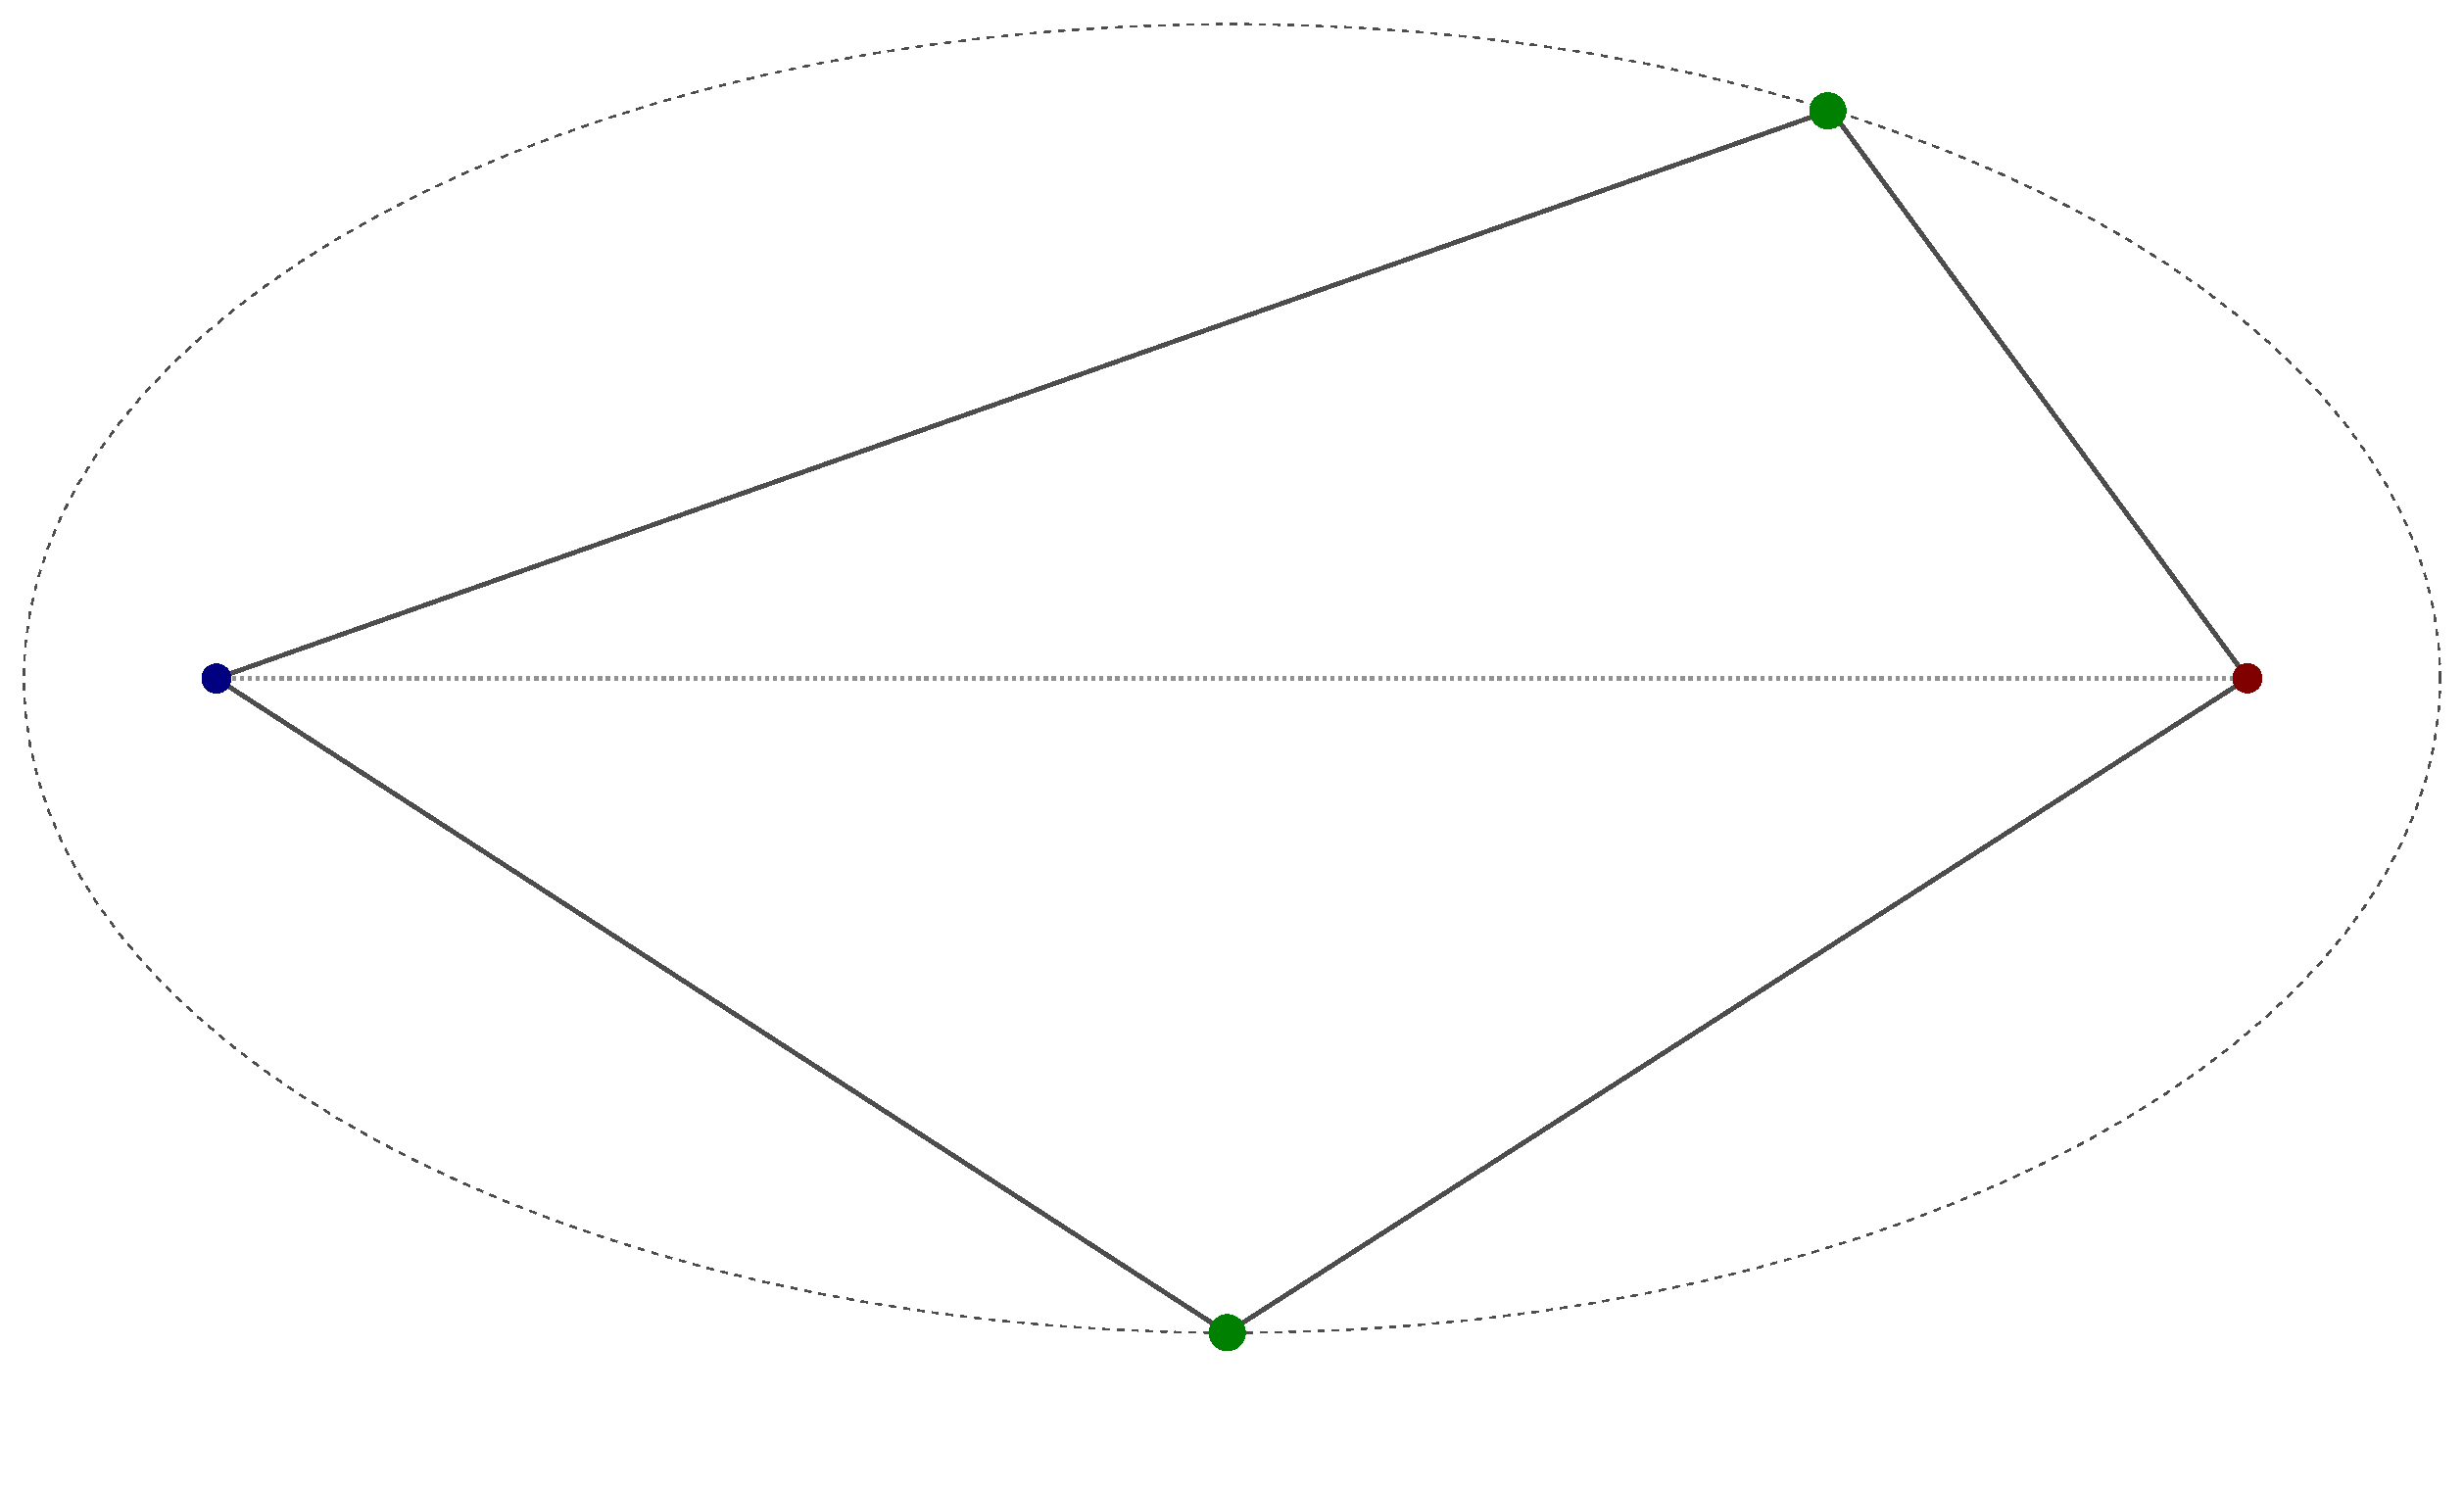
\includegraphics[width=0.8\linewidth]{Elliptic_Curve.pdf}
    \caption{Elliptic trace of possible target positions as measured by a bistatic radar system}
    \label{fig:Elliptic_Curve}
\end{figure}

As a consequence of this, bistatic radar requires additional measurements in order to locate a target accurately. For example, one can use the doppler shift of the object in order to determine its velocity, and thus pinpoint its position on the elliptic trace. Alternatively, multiple bistatic radar systems can be used simultaneously, and the intersection of the resultant ellipses then indicates the target's location. This latter approach is termed a \emph{multistatic} radar, and is shown in figure~\ref{fig:Multistatic_Geometry}. Note that a multistatic arrangement is loosely defined, and may actually comprise of multiple bistatic and/or monostatic radar systems.

Notice that in passive radar situations, the illuminator of opportunity will never be collocated with the receiver; thus, such systems are always at least bistatic, or are otherwise multistatic. Kuschel and O'Hagan have suggested that the convenience and simplicity of active monostatic radars, especially due to the adoption of the duplexer, shifted focus away from passive radar systems in the years after the Second World War~\cite{kuschel-hagan-history}.

Some attention was renewed to passive systems in around 1980, and has increased ever since. This is particularly in line with the advancement of signal jamming techniques, with the potential to cripple existing active radars.

\subsection{Advantages \& Disadvantages of Passive Radar}
Passive radar has a host of advantages over its active counterpart, as well as a handful of drawbacks.

\subsubsection{Advantages}
Firstly, since passive radar systems use existing transmitters, no additional \gls{em} spectrum allocation is required for their operation. This is particularly relevant in the current technological context, where spectrum is fiercely sought after, often involving huge sums of money and political lobbying. Deploying an active radar system requires licensing for its utilized frequency bands; whereas a passive radar can simply hitchhike off an already-licensed transmission.

Moreover, not only can a passive radar operate without licensing requirements---thus saving costs---it can also operate without the cost of transmitting enormous amounts of power. A useful radar transmitter may need to transmit kilowatts of power, which naturally has an associated electrical cost.

These cost savings make passive radar an interesting case-study in particular for poorer nations. 

One of the major attractions of passive radar is in a military context: since no additional \gls{em} energy is emitted, the receiver location remains covert. Some scholars have shown that this is not completely foolproof, but it certainly poses an advantage over the highly-noticeable active radar systems. Passive radar systems also have a high resistance to EM countermeasures. Also counter-counter-stealth, due to low-observable targets and forward scatter.

\cite{o2009passive}

These benefits exist outside of a military domain, too. A case study for this is Peralex Electronics' work done for the Square Kilometer Array (SKA) project. The SKA is a massive radio-telescope. Telescopes are so sensitive that the surrounding zones need to be largely electromagnetically clean within the telescope's operating bands. Unfortunately, planes flying past (and weather radars) fly over and can damage the receivers. However, using an active radar system to detect these planes would be pointless---as the system itself would interfere with the telescopes.

The solution here was using a passive radar system hitchhiking on surrounding FM broadcasts. The FM band falls below the telescope's operating range.

\subsubsection{Disadvantages}

- No control over the transmitter

- Transmitted waveform not designed for radar

- DSI

% -------- DIGITAL BROADCASTING --------
\section{Digital Broadcasting}
When considering the innumerable technological advancements of the past century, one cannot overlook the enormous impact of wireless broadcasting. The advent of mass communication, first via radio and later via television, has undoubtedly shaped our culture, our politics, and frankly, our entire lives. The ability for many, many people to receive the same message---be it audio, visual, or textual---certainly built the stage for the zeitgeist of the 21st-century. While this project revolves nominally around passive radar, most of it, in fact, relates to digital broadcasting. The end goal remains as the use of the latter in the context of the former, but the success of digital broadcasting-based passive radar is intimately related to the success of digital broadcasting itself.

\subsection{History of Digital Broadcasting}
Around the same time that H\"ulsmeyer \emph{et al.} were experimenting with early radar systems, there was development occurring in wireless \emph{audio} transmissions. In 1900, Reginald Fessenden successfully demonstrated an \gls{am} transmission, over a distance of 1.6km, using his so-called \emph{radiotelephone}. In the decades that followed, radio broadcasting became a staple of (Western) culture. By the 1920s, \gls{am} radios were rolling out to everyday households, and new levels of mass communication were achieved. Who can imagine what the Second World War would have been like in the absence of national briefings?

All of the investigations hitherto were in analogue broadcasting. The computational power of the early computers was simply inadequate for the demands of digital transmission. Nevertheless, as computers matured, the scene was set for change: investigations into digital broadcasting techniques began. In the 1980s, research began on the Eureka 147 project in Europe, which later became the \gls{dab} standard---the focus of this report. Patents for digital radio devices began appearing in the mid-1980s.

(Note the importance of OFDM)

Now, in 2020, the technology is far more mature, but global adoption is still mixed. In some states, digital transmissions have completely displaced analog counterparts, such as Germany's nationwide implementation of digital television. In other states, however, progress is slower. In a South African context, the \gls{icasa} promised to shut off analog broadcasts in 2011. At present, this has still not occurred.

\subsection{Advantages \& Disadvantages of Digital Broadcasting}
The benefits and drawbacks of digital broadcasting depend largely on the particular use case. However, there are a handful of consistent advantages, as well as disadvantages.

\subsubsection{Advantages}
- More efficient bandwidth allocation
- Perfectly decodable video and audio (robust to errors)
- Single Frequency Networks

\subsubsection{Disadvantages}

\subsection{Digital Broadcasting Standards \& Adoption}
There are a host of digital broadcasting standards, spanning a host of use-cases and contexts. To complicate matters further, standards vary by country.

\begin{itemize}
    \item Video standards
        \begin{itemize}
            \item Digital Video Broadcasting (DVB) \\
            This is the most adopted standard, and the most relevant in a South African context.
            \item Advanced Television Systems Committee
        \end{itemize}
    \item Audio standards
        \begin{itemize}
            \item Digital Audio Broadcasting (DAB) \\
            \item 
        \end{itemize}
\end{itemize}

% -------- IMPLEMENTATIONS --------
\section{Digital Broadcasting-based Passive Radar}
With the foundations of both passive radar and digital broadcasting presented, it is now interesting to look at the literature relevant to this project: using digital broadcasting signals in the context of a passive radar chain. When passive radar first started resurfacing in the early 1990s, most---if not all---of the work was being done with \gls{fm} signals. This is logical, as \gls{fm} signals were by-far the most ubiquitous radio format globally at that time. Since then, development has branched out into using other signal modulation types, even using WiFi and 

\subsection{Advantages}
\subsection{Existing Implementations}




% ----------------------------------------------------
\ifstandalone
\bibliography{../Bibliography/References.bib}
\printnoidxglossary[type=\acronymtype,nonumberlist]
\fi
\end{document}
% ----------------------------------------------------